\documentclass{article}
\usepackage[T2A]{fontenc}
\usepackage[utf8]{inputenc}
\usepackage[russian]{babel}
\usepackage{graphicx}
\usepackage[left = 3cm, right = 2cm, top = 2cm]{geometry}
\usepackage{wrapfig}
\usepackage{amsmath}
\usepackage{float}
%\graphicspath{ {./images/} }

\author{Александр Романов Б01-107}
\date{}
\title{Лабораторная работа №2.2.1 \newline Исследование взаимной диффузии газов}

\begin{document}
\maketitle
\newpage
\section{Введение}

\textbf{Цель работы:} 1) регистрация зависимости концентрации гелия
в воздухе от времени с помощью датчиков теплопроводности при
разных начальных давлениях смеси газов; 2) определение коэффи-
циента диффузии по результатам измерений.\\
\textbf{В работе используются:} измерительная установка; форвакуум-
ный насос; баллон с газом (гелий); манометр; источник питания;
магазин сопротивлений; гальванометр; секундомер.

\section {Работа}

Запишем геометрические параметры установки:
\begin{figure}[H]
    \centering
    \begin{tabular}{|c|c|c|c|c|}
        \hline
        $V_1, \text{см}:2$&$V_2, \text{см}^2$&$\frac{L}{S}, \frac{1}{\text{см}}$&$P_{\text{гел}}$&$P_{\text{возд}}$ \\\hline
        $800\pm5$&$800\pm5$&$15.0\pm0.1$&$0.2P_{\text{раб}}$&$1.75P_{\text{раб}}$ \\\hline
    \end{tabular}
\end{figure}

Измерения проведём для 4 разных значений $P_{\text{раб}}$: 40, 80, 120 и 160 торр.
Для каждого из давлений построим график в координатах $
ln(U)$, $t$. Показания вольтметра были в мВ, затем обезразмерены. $t$ измерялось в секундах.
\begin{enumerate}
    \item \textbf{$P_{\text{раб}} = 40\text{торр}$}:
        \begin{figure}[H]
            \centering
            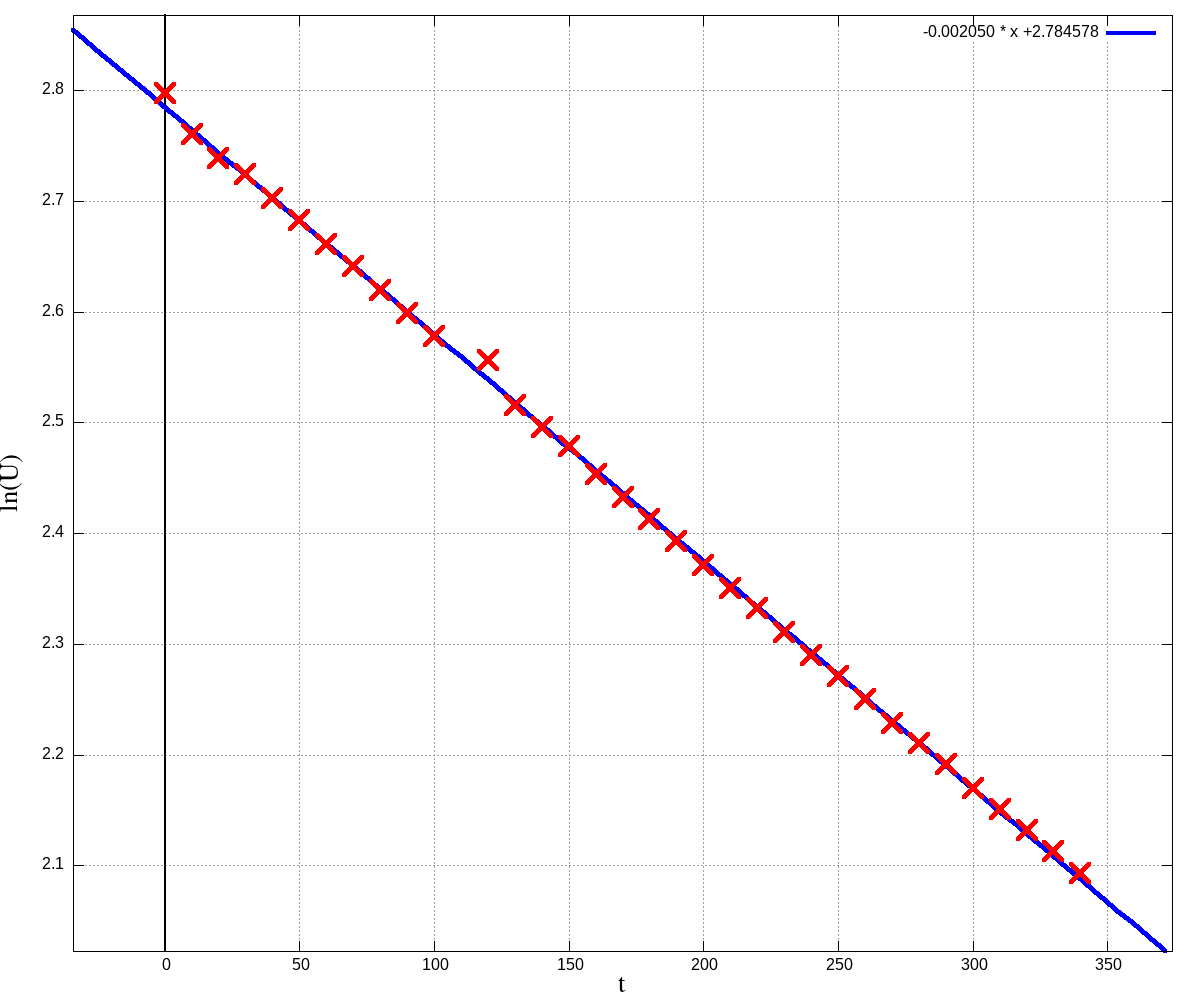
\includegraphics[width=0.8\textwidth]{graph1.png}
        \end{figure}

        В полученной линейной зависимости вида ($y = kx + b$):\\
        $k = -0.00205 \pm 7.6\cdot 10^{-6}$, $b = 2.785 \pm 7.8\cdot10^{-4}$

        \item \textbf{$P_{\text{раб}} = 80\text{торр}$}:
    \begin{figure}[H]
        \centering
        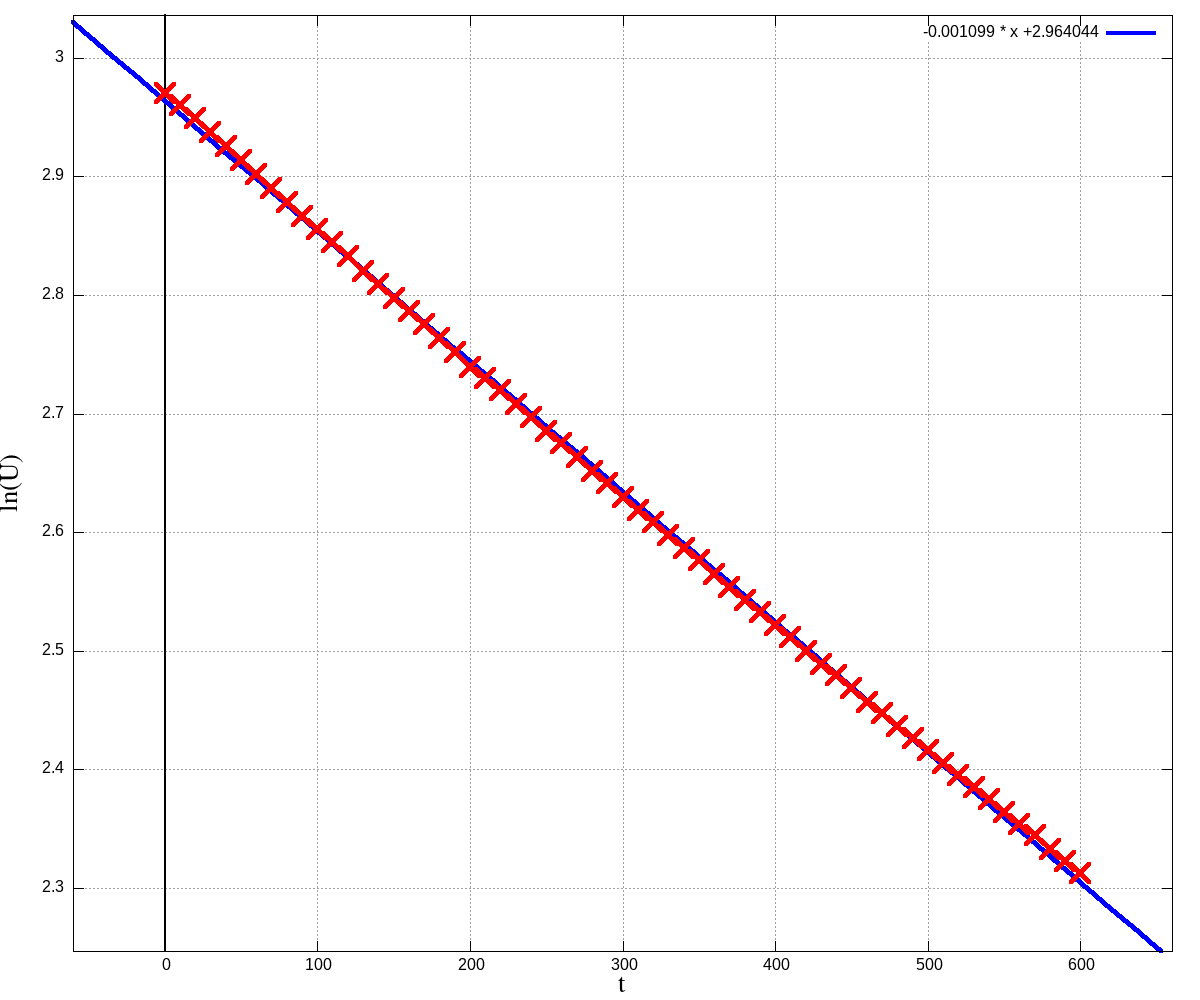
\includegraphics[width=0.8\textwidth]{graph2.png}
    \end{figure}

    В полученной линейной зависимости вида ($y = kx + b$):\\
    $k = -0.001099 \pm 2.8\cdot 10^{-6}$, $b = 2.964 \pm 4.9\cdot10^{-4}$

    \item \textbf{$P_{\text{раб}} = 120\text{торр}$}:
    \begin{figure}[H]
        \centering
        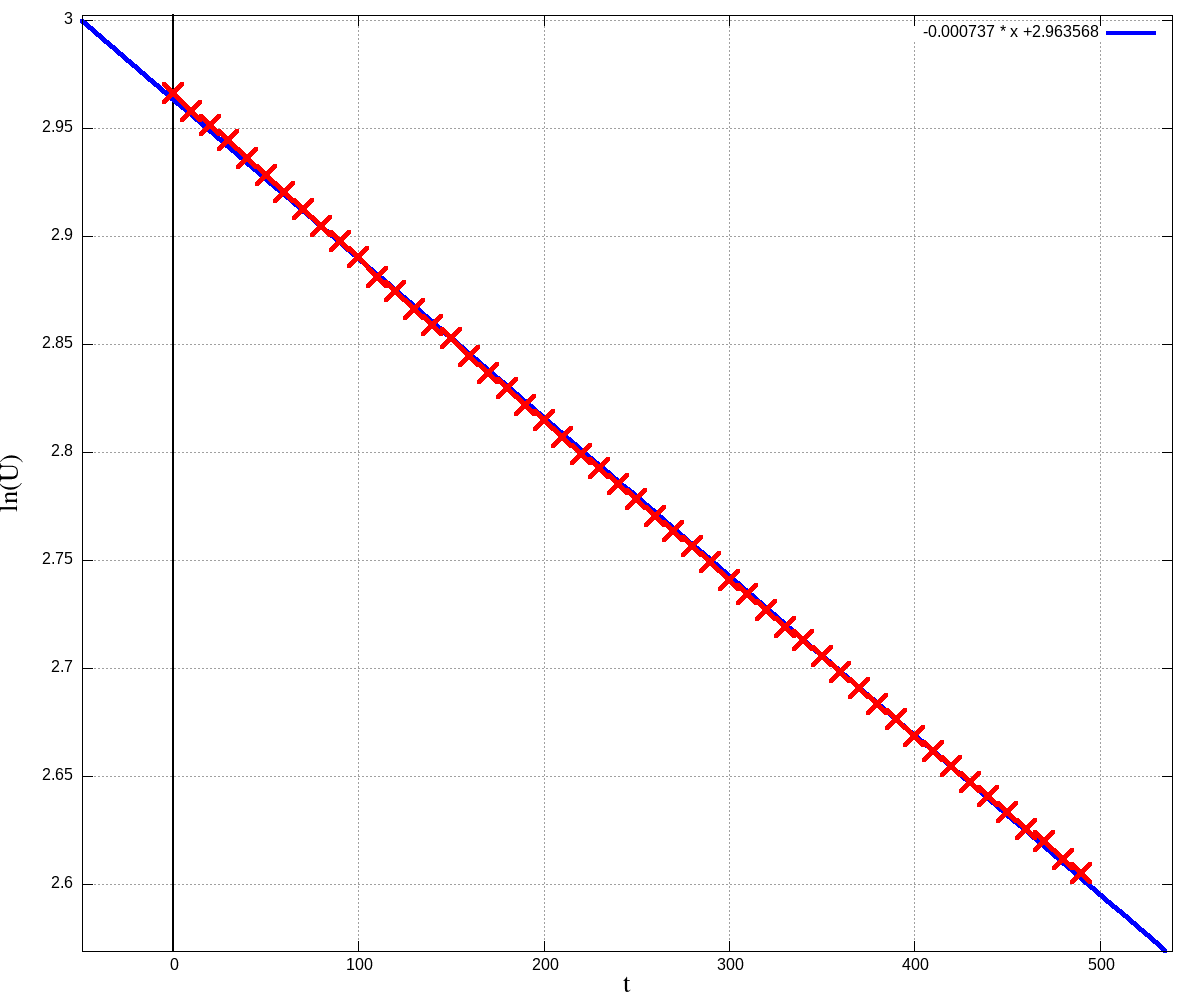
\includegraphics[width=0.8\textwidth]{graph3.png}
    \end{figure}

    В полученной линейной зависимости вида ($y = kx + b$):\\
    $k = -0.000737 \pm 1.4\cdot 10^{-6}$, $b = 2.964 \pm 2.0\cdot10^{-4}$

    \item \textbf{$P_{\text{раб}} = 160\text{торр}$}:
    \begin{figure}[H]
        \centering
        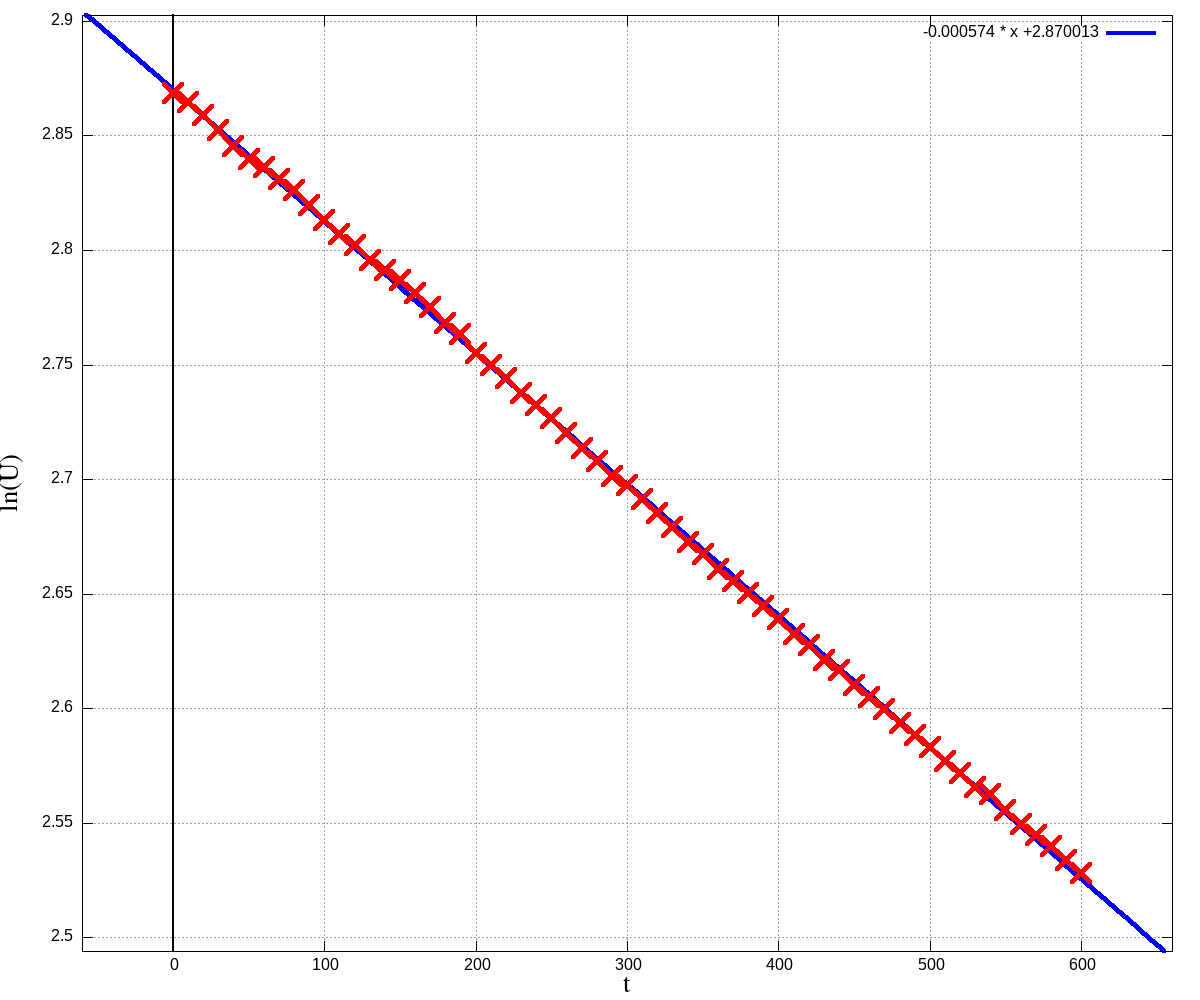
\includegraphics[width=0.8\textwidth]{graph4.png}
    \end{figure}

    В полученной линейной зависимости вида ($y = kx + b$):\\
    $k = -0.000574 \pm 1.1\cdot 10^{-6}$, $b = 2.87 \pm 1.9\cdot10^{-4}$
\end{enumerate}

Найдём коэффициенты взаимной диффузии газов из формулы:
\[D = \frac{L}{S}\cdot\frac{V_1V_2}{V_1 + V_2}\cdot\frac{1}{\tau}\]
Переведя единицы измерения в СИ получим:
\begin{figure}[H]
    \centering
    \begin{tabular}{|c|c|c|c|}
        \hline
        $D_1, \frac{\text{м}^2}{c}$&$D_2, \frac{\text{м}^2}{c}$&$D_3, \frac{\text{м}^2}{c}$&$D_4, \frac{\text{м}^2}{c}$\\\hline
        0.00123&0.00066&0.00044&0.00034\\\hline
    \end{tabular}
\end{figure}
Построи график зависимости $D\left(\frac{1}{P}\right)$:
\begin{figure}[H]
    \centering
    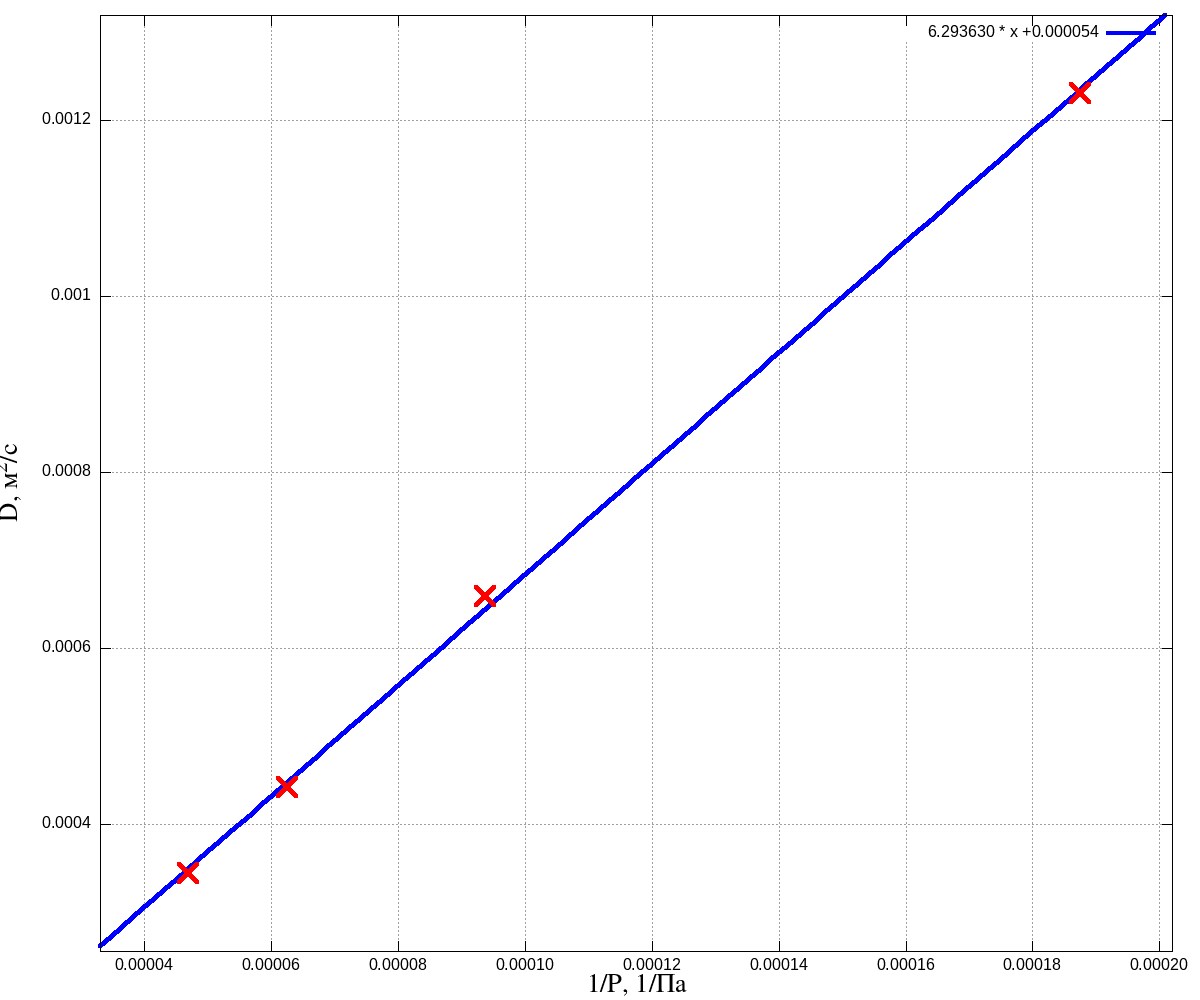
\includegraphics[width=0.8\textwidth]{graphD.png}
\end{figure}

В полученной линейной зависимости вида ($y = kx + b$):\\
    $k = 6.294 \pm 0.08 \frac{\text{м}^2\text{Па}}{c}$, $b = 5.4\cdot10^{-5} \pm 4.3\cdot10^{-6} \frac{\text{м}^2}{c}$
Расчитаем коэффициент диффузии при атмосферном давлении:
\[ D_{P_0} = 1.12 \frac{\text{см}^2}{c} \]

\section{Выводы}
\begin{enumerate}
    \item 
Итак, по произведённным нами расчётам мы получили зависимости концентрации гелия в воздухе от времени.
И по полученным угловым коэффициентам посчитали коэффициент вазимной диффузии He - воздух для 4-х
различных значений давлеия.
    \item
Мы получили зависимость коэффициента диффузии от давления и посчитали таким образом этот коэффициент 
для атмосферного давления. Полученный результат оказался достаточно близким к табличному ($D_{P_0} = 0.62\frac{\text{см}^2}{c}$)
\end{enumerate}

\end{document}